%% The following is a directive for TeXShop to indicate the main file
%%!TEX root = diss.tex

\chapter{Engineering Organic Molecular Energy Levels}
\label{ch:oled}

% importance of engineering energy levels (optical gap, colour, applications in biomedical imaging?)
% can be done by using functional groups
% can examine the single molecule effects of functionalization 

The energy levels of organic semiconducting molecules determines the electronic and optical properties of the molecule. For different applications, there are different optimal energy level alignments. Through variation in the design of organic molecules, possible through organic synthesis techniques, the energy levels of the organic semiconductor can be engineered. This is realised through the addition of functional groups to an organic molecule or polymer \citep{schwarze2016band, VanMullekom2001}. In particular, this chapter will discuss the functionalization of \ac{HMAT} with various acceptor complexes, with \ac{HMAT} acting as the donor, and the resulting molecular orbitals and their energy levels. I will also discuss the attempts of \ac{STML} experiments on these \ac{HMAT} derivative molecules.




\section{Introduction to HMAT}

% talk about the HMAT molecule, where it came from
% why we are interested?
% possible functionalization of molecules

\Acf{HMAT} is a highly stable and planar molecule with interesting optoelectronic properties. With a theoretical HOMO-LUMO gap of \SI{4.45}{eV}, \ac{HMAT} is a good electron donor molecule and a deep blue-violet fluorophore \cite{Tonge2020} (\autoref{fig:oled:dft-hmat}). With a rigid planar structure, electrons in \ac{HMAT} have enhanced $\pi$-conjugation, giving it a high quantum photoluminescent efficiency, along with a high photon absorption cross-section \citep{Makarov2012}. Additionally, functionalized \ac{HMAT} derivatives have demonstrated optical effects such as thermally activated triplet exicton formation \citep{Chen2017}, and two-photon excited fluorescence \citep{Fang2012,Paisley2020}, making these molecules candidates for \ac{OLED} and biological imaging applications. 

\begin{figure} [h]
    \centering
    %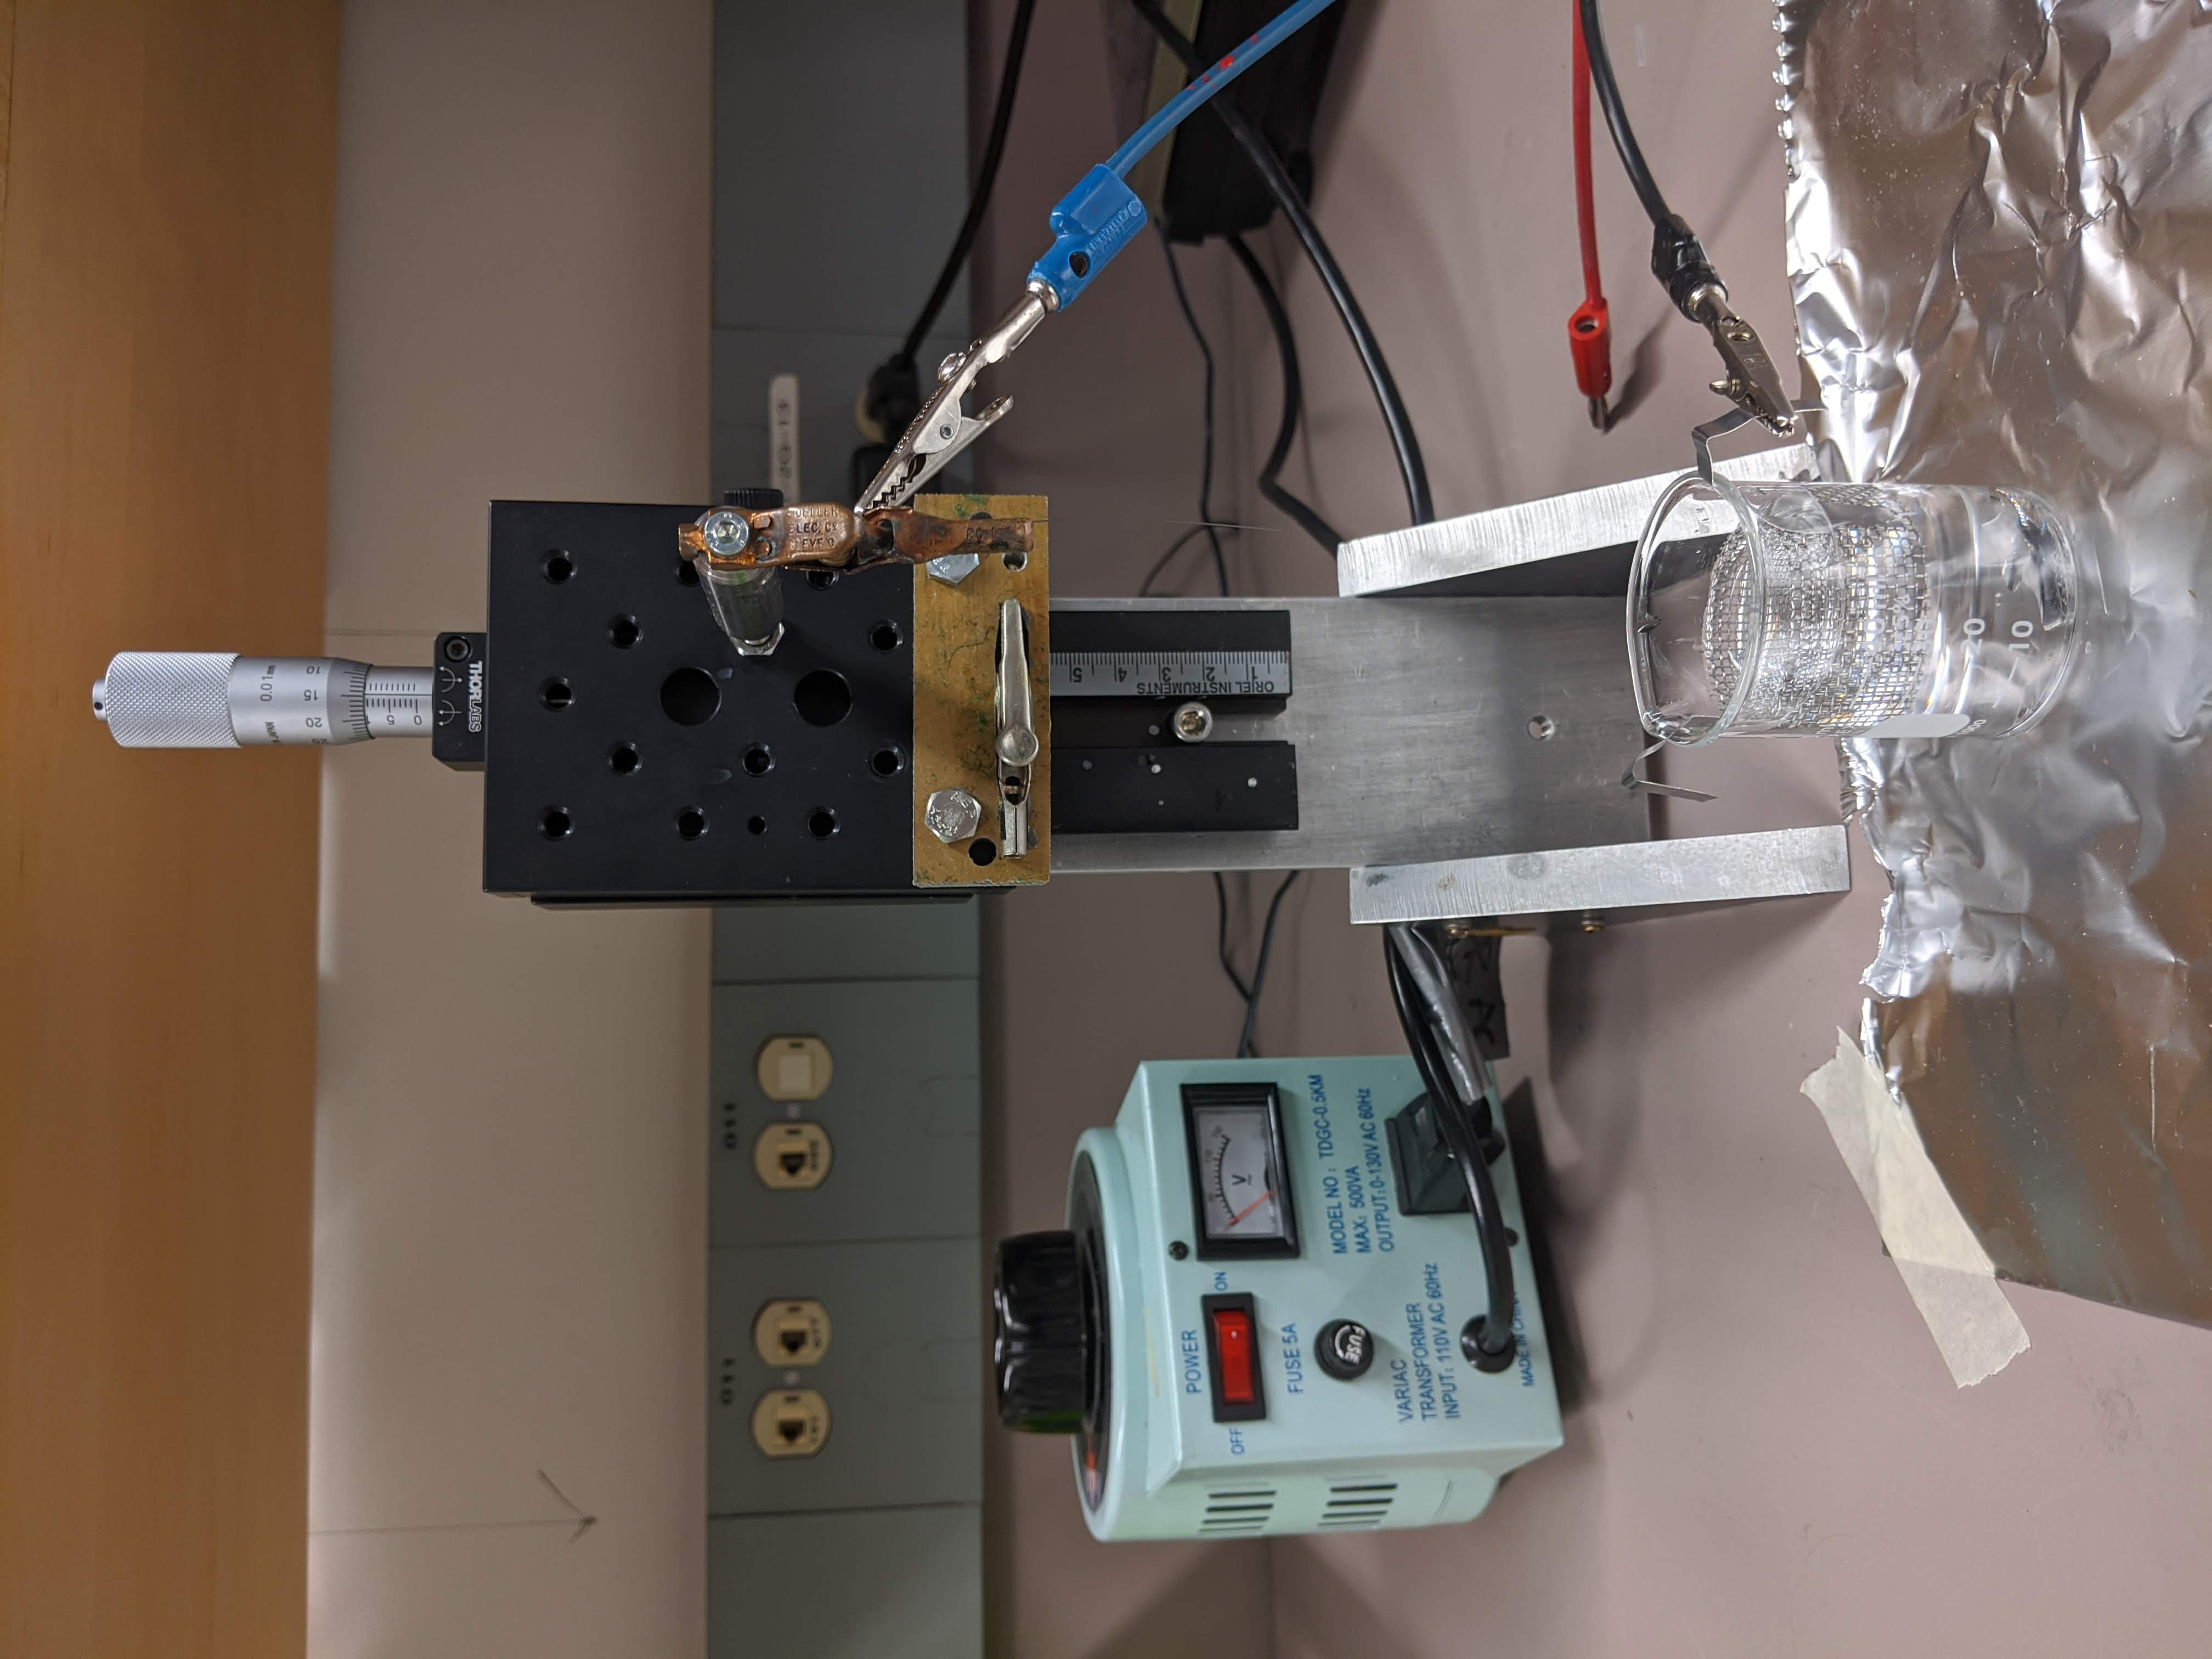
\includegraphics[width=3in,angle=-90]{pictures/etching.jpg}
    \caption{\FIXME{DFT of HMAT alone}}
    \label{fig:oled:dft-hmat}
\end{figure}

Being relatively difficult to synthesize, the functionalized \ac{HMAT} derivatives were not available commercially and was provided by our collaborators in the chemistry department at \ac{UBC}. We examined three different \ac{HMAT} derivative molecules: \ac{HMAT-O}, \ac{HMAT-TZ}, and \ac{HMAT-HZ}. The chemical structure of each is shown in \autoref{fig:oled:hmat-derivatives}. All prior studies on \ac{HMAT} and its functionalized derivatives were in chemical ensembles with conventional analytical techniques. With \ac{SPM}, for each functional group, we can visualize the sub-molecular spatial distribution of the orbitals, and measure the energy levels of the single molecule. 

% are relatively difficult to synthesize molecules, that are not commercially available. Provided by our collaborators in the chemistry department at UBC, they have only been examined using conventional analytical chemistry techniques as a chemical ensemble. Here, we present a submolecular study of molecules that are derived from HMAT, a highly stable molecule with a large HOMO-LUMO gap capable of efficiently emitting ultraviolet light. By adding functional groups of increasing electronegativity, the HOMO-LUMO gap and the colour of emission can be tuned. 


\begin{figure} [h]
    \centering
    %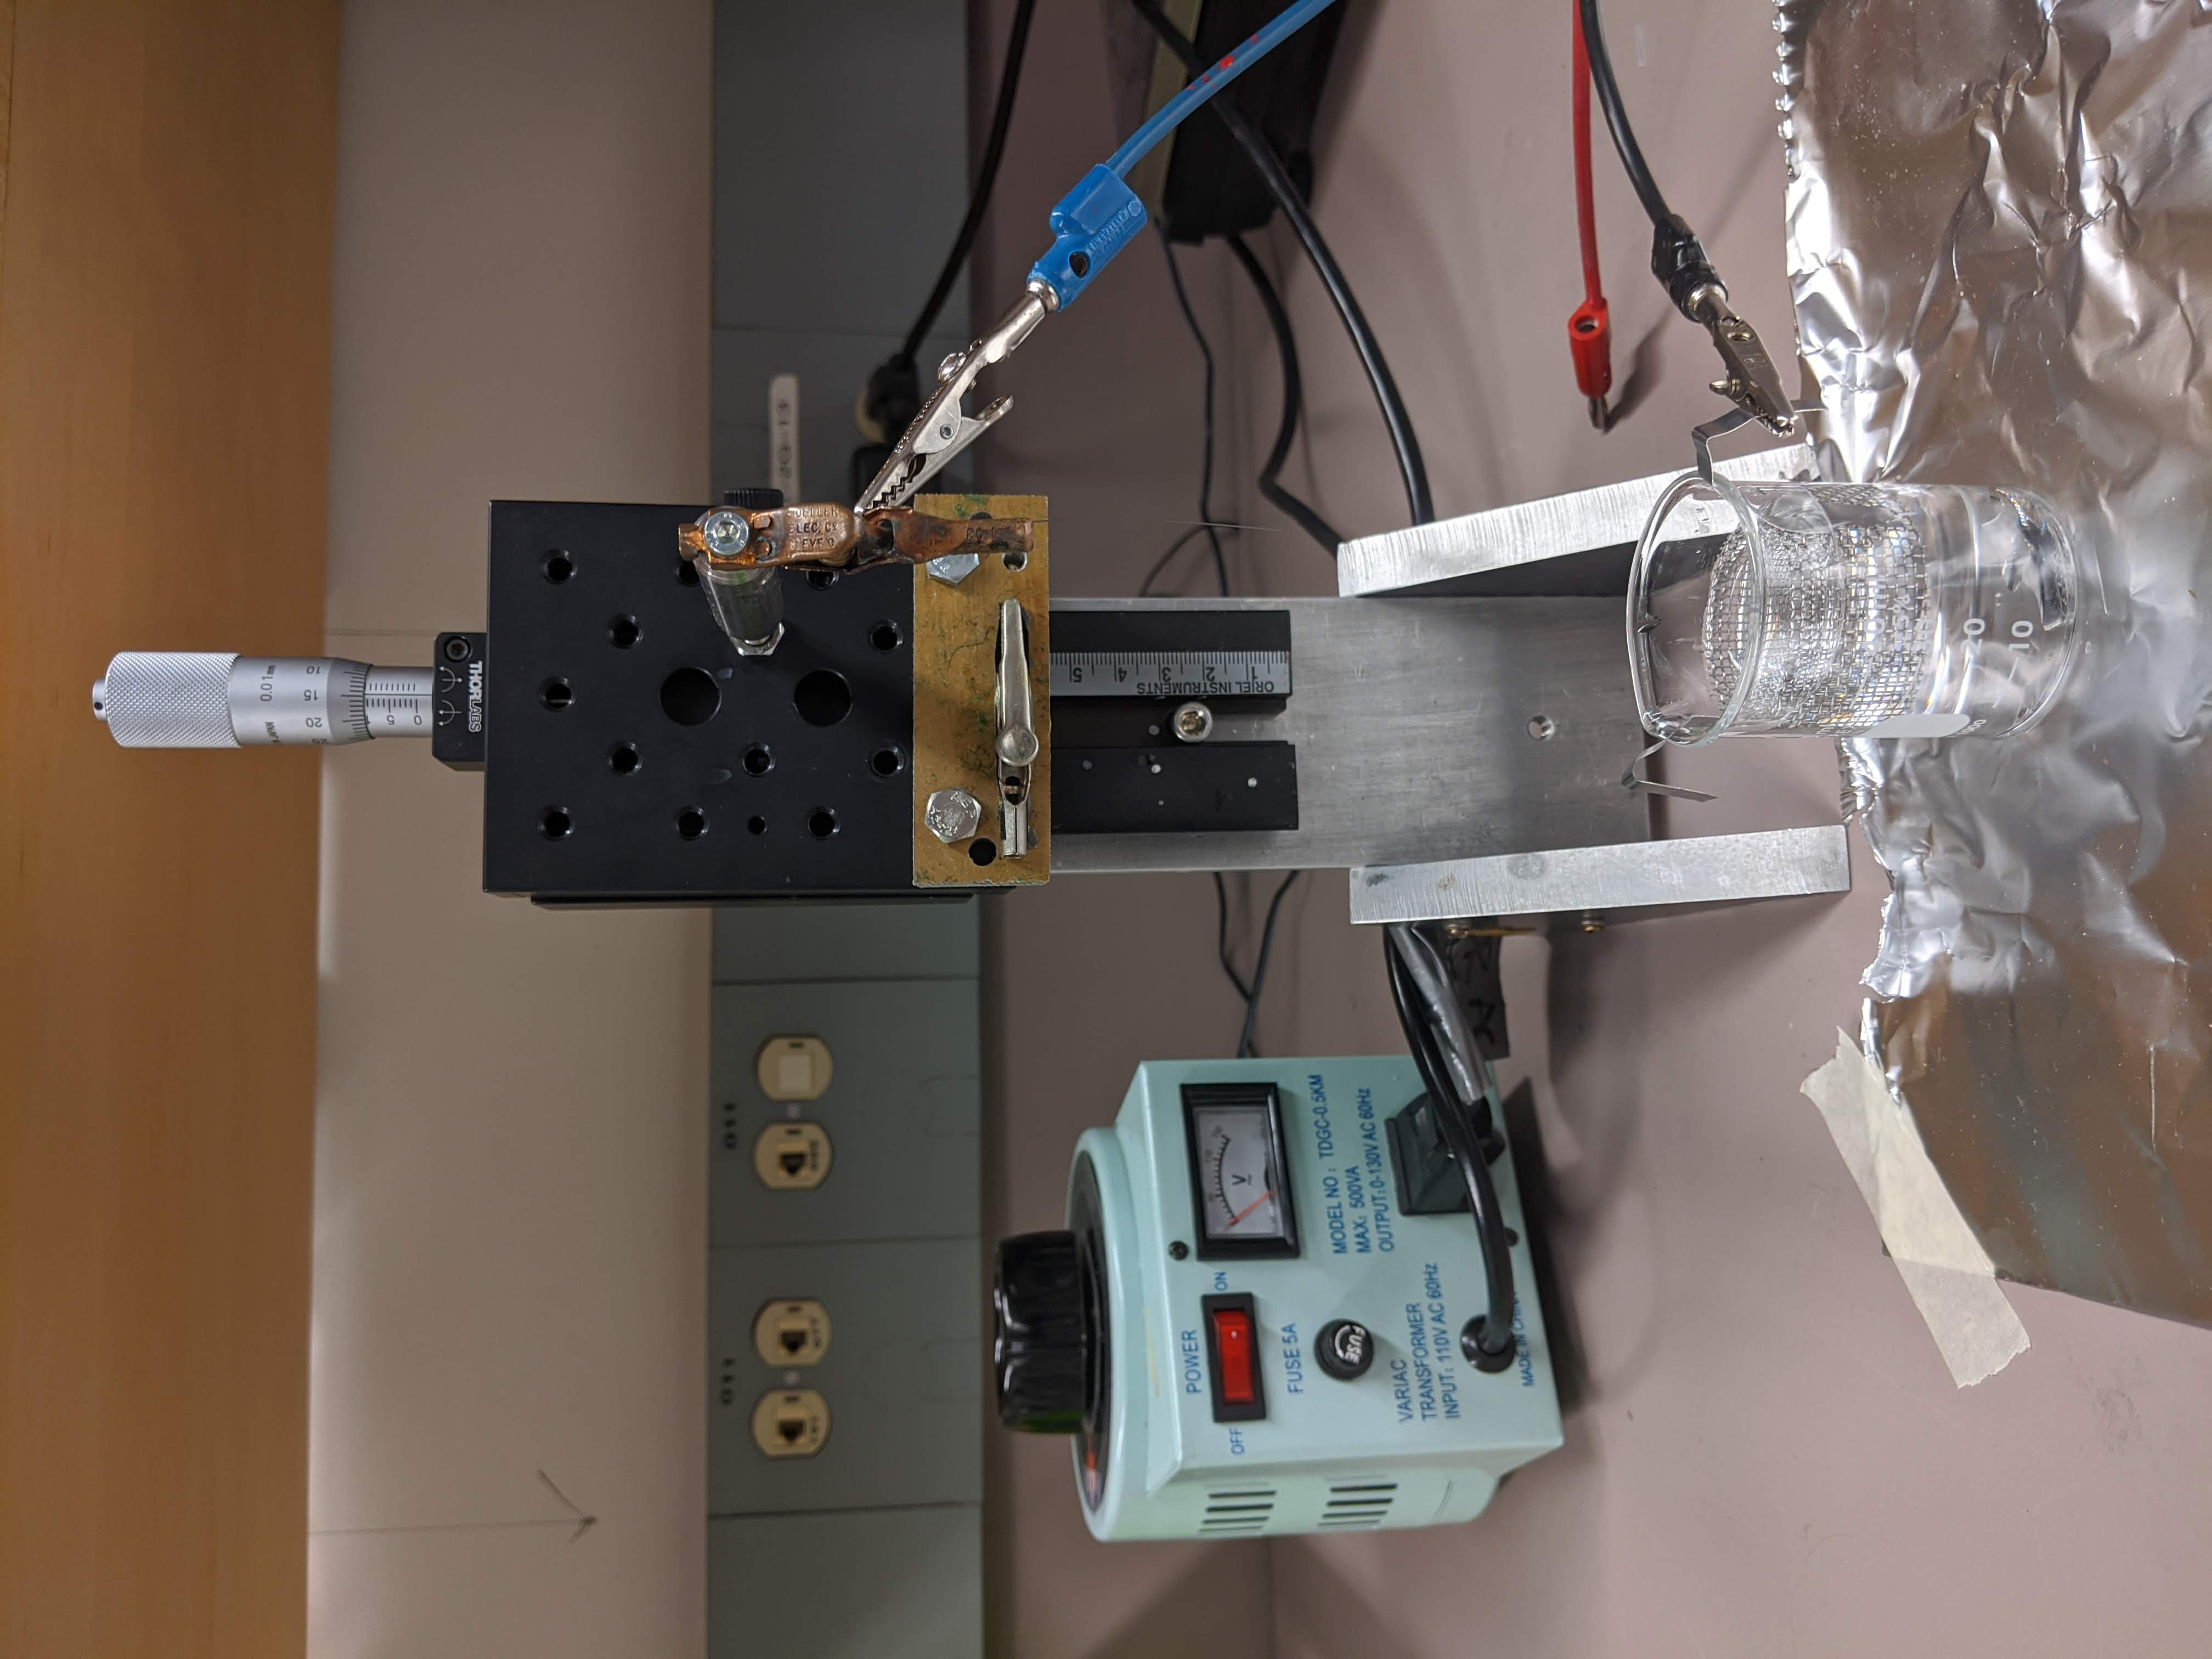
\includegraphics[width=3in,angle=-90]{pictures/etching.jpg}
    \caption{\FIXME{chemical structures of hmat and derivatives}}
    \label{fig:oled:hmat-derivatives}
\end{figure}




\section{{STM}/{STS} study of HMAT derivatives}

The molecules were deposited onto the bare Ag(111) surface, and probed with a Pt/Ir tip dipped in silver. While the \ac{HMAT} molecule is highly stable, the attached functional groups were fragmented at high deposition temperatures. Large area \ac{STM} scans showed an abundance of fragments on the surface for each molecule deposition, even after repeated degassing (\autoref{fig:oled:hmat-frag}). 

\begin{figure} [h]
    \centering
    %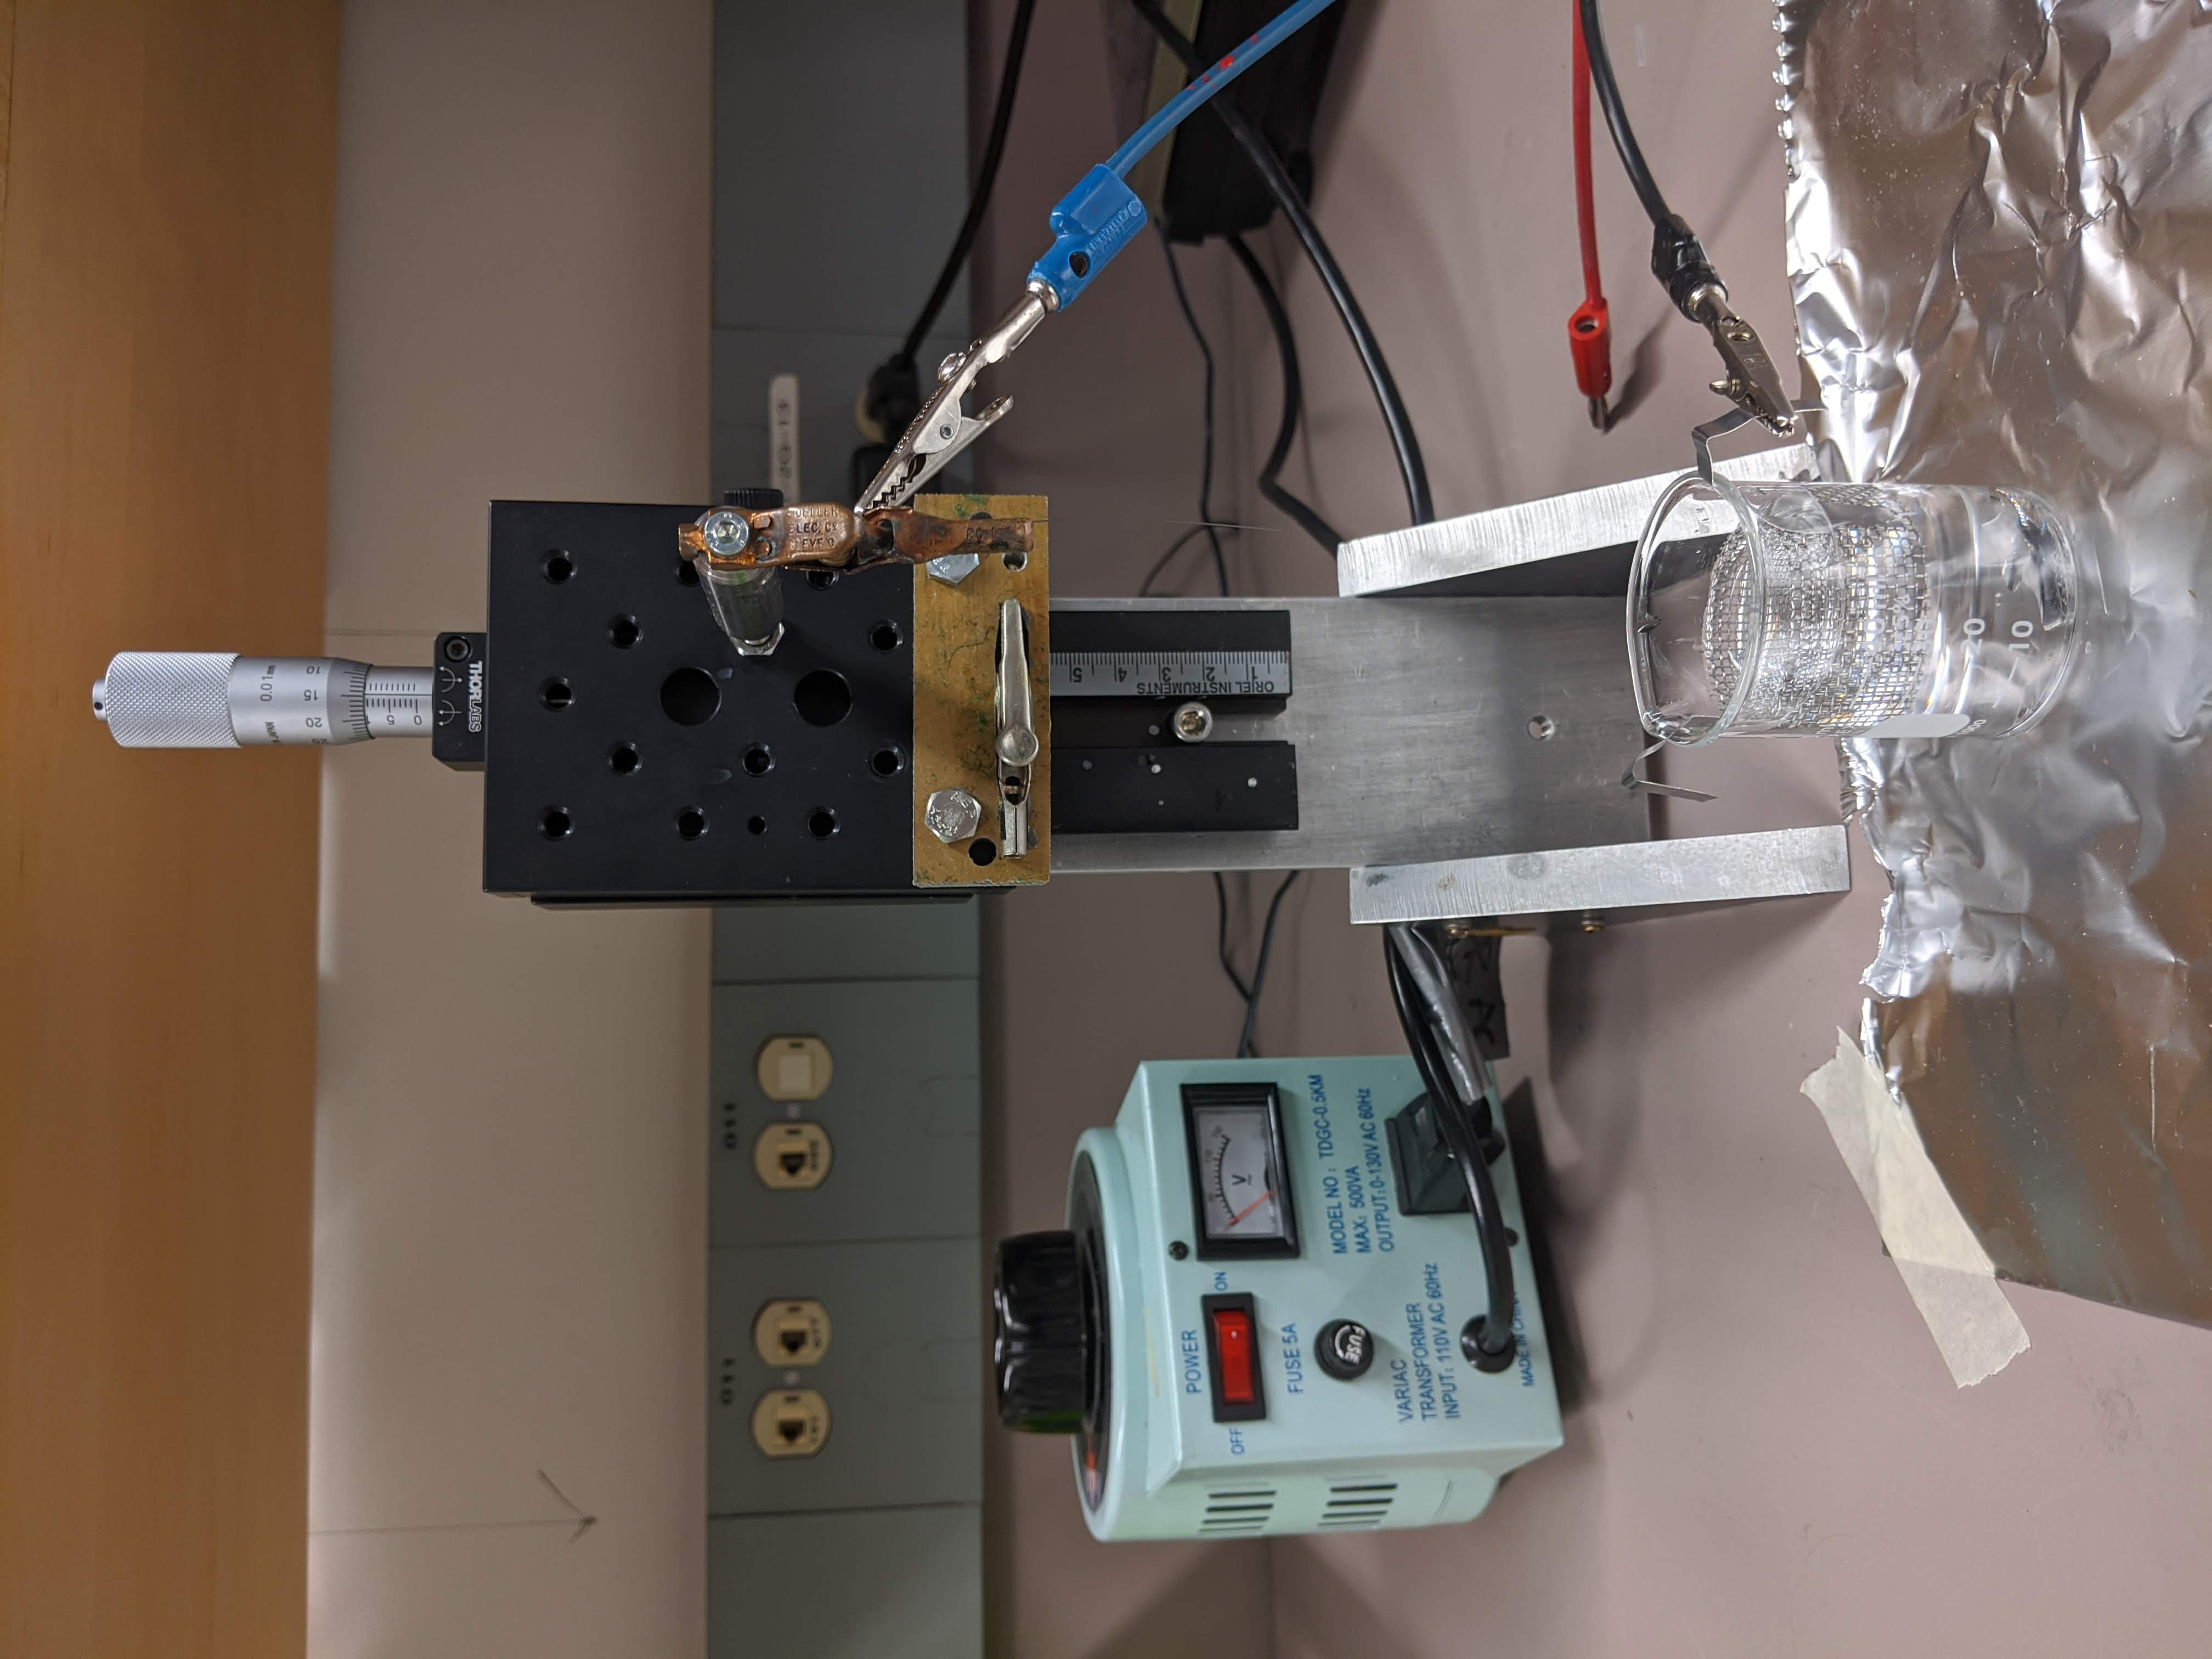
\includegraphics[width=3in,angle=-90]{pictures/etching.jpg}
    \caption{\FIXME{show the fragmented images}}
    \label{fig:oled:hmat-frag}
\end{figure}

Fortunately, intact molecules were found with still attached functional groups. The molecules were scanned, and a pixel-by-pixel \ac{STS} grid was performed on the molecules on Ag(111). Taking the normalized differential conductance, the \ac{LDOS} was plotted as a function of energy, and the \ac{HOMO} and \ac{LUMO} orbitals were visualized spatially. \ac{DFT} calculations were performed for each of the \ac{HMAT} derivative molecules, and used as comparison to the experimental results. The results for HMAT-O, HMAT-TZ, and HMAT-HZ are shown in Figures \ref{fig:oled:hmat-o}, \ref{fig:oled:hmat-tz}, and \ref{fig:oled:hmat-hz}, respectively. 

\begin{figure} [h]
    \centering
    %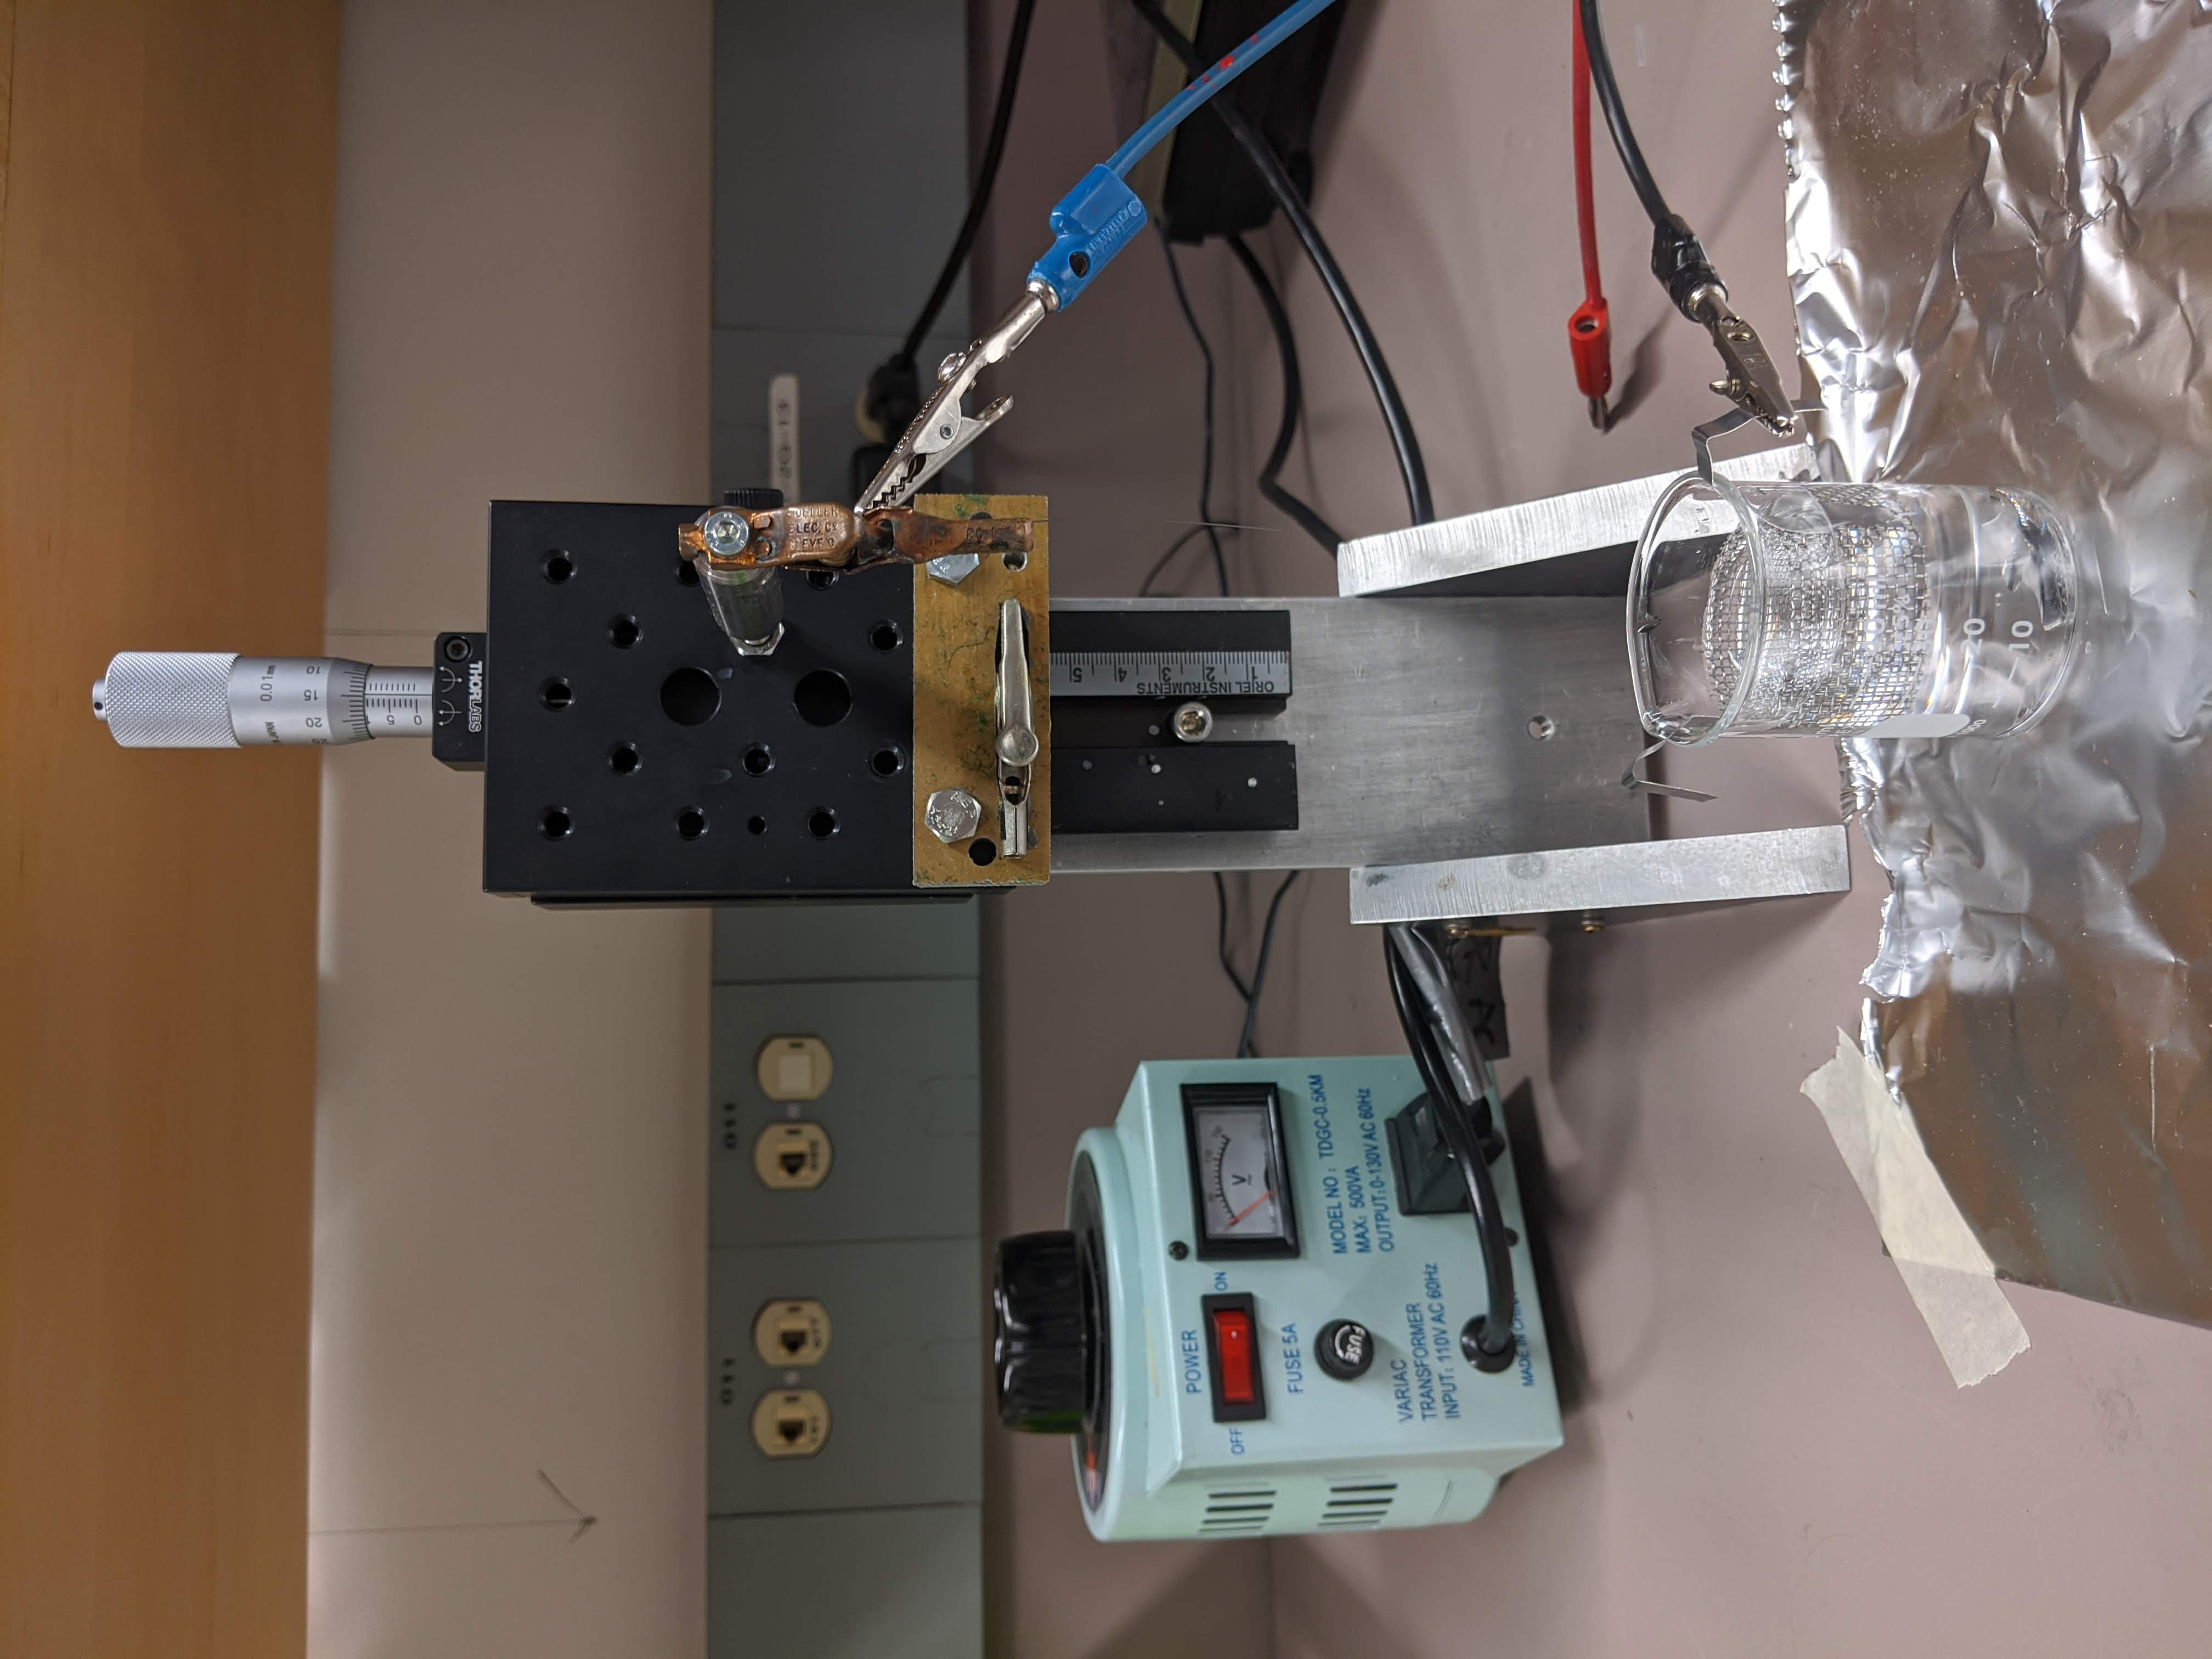
\includegraphics[width=3in,angle=-90]{pictures/etching.jpg}
    \caption{\FIXME{show hmat-o data}}
    \label{fig:oled:hmat-o}
\end{figure}

\begin{figure} [h]
    \centering
    %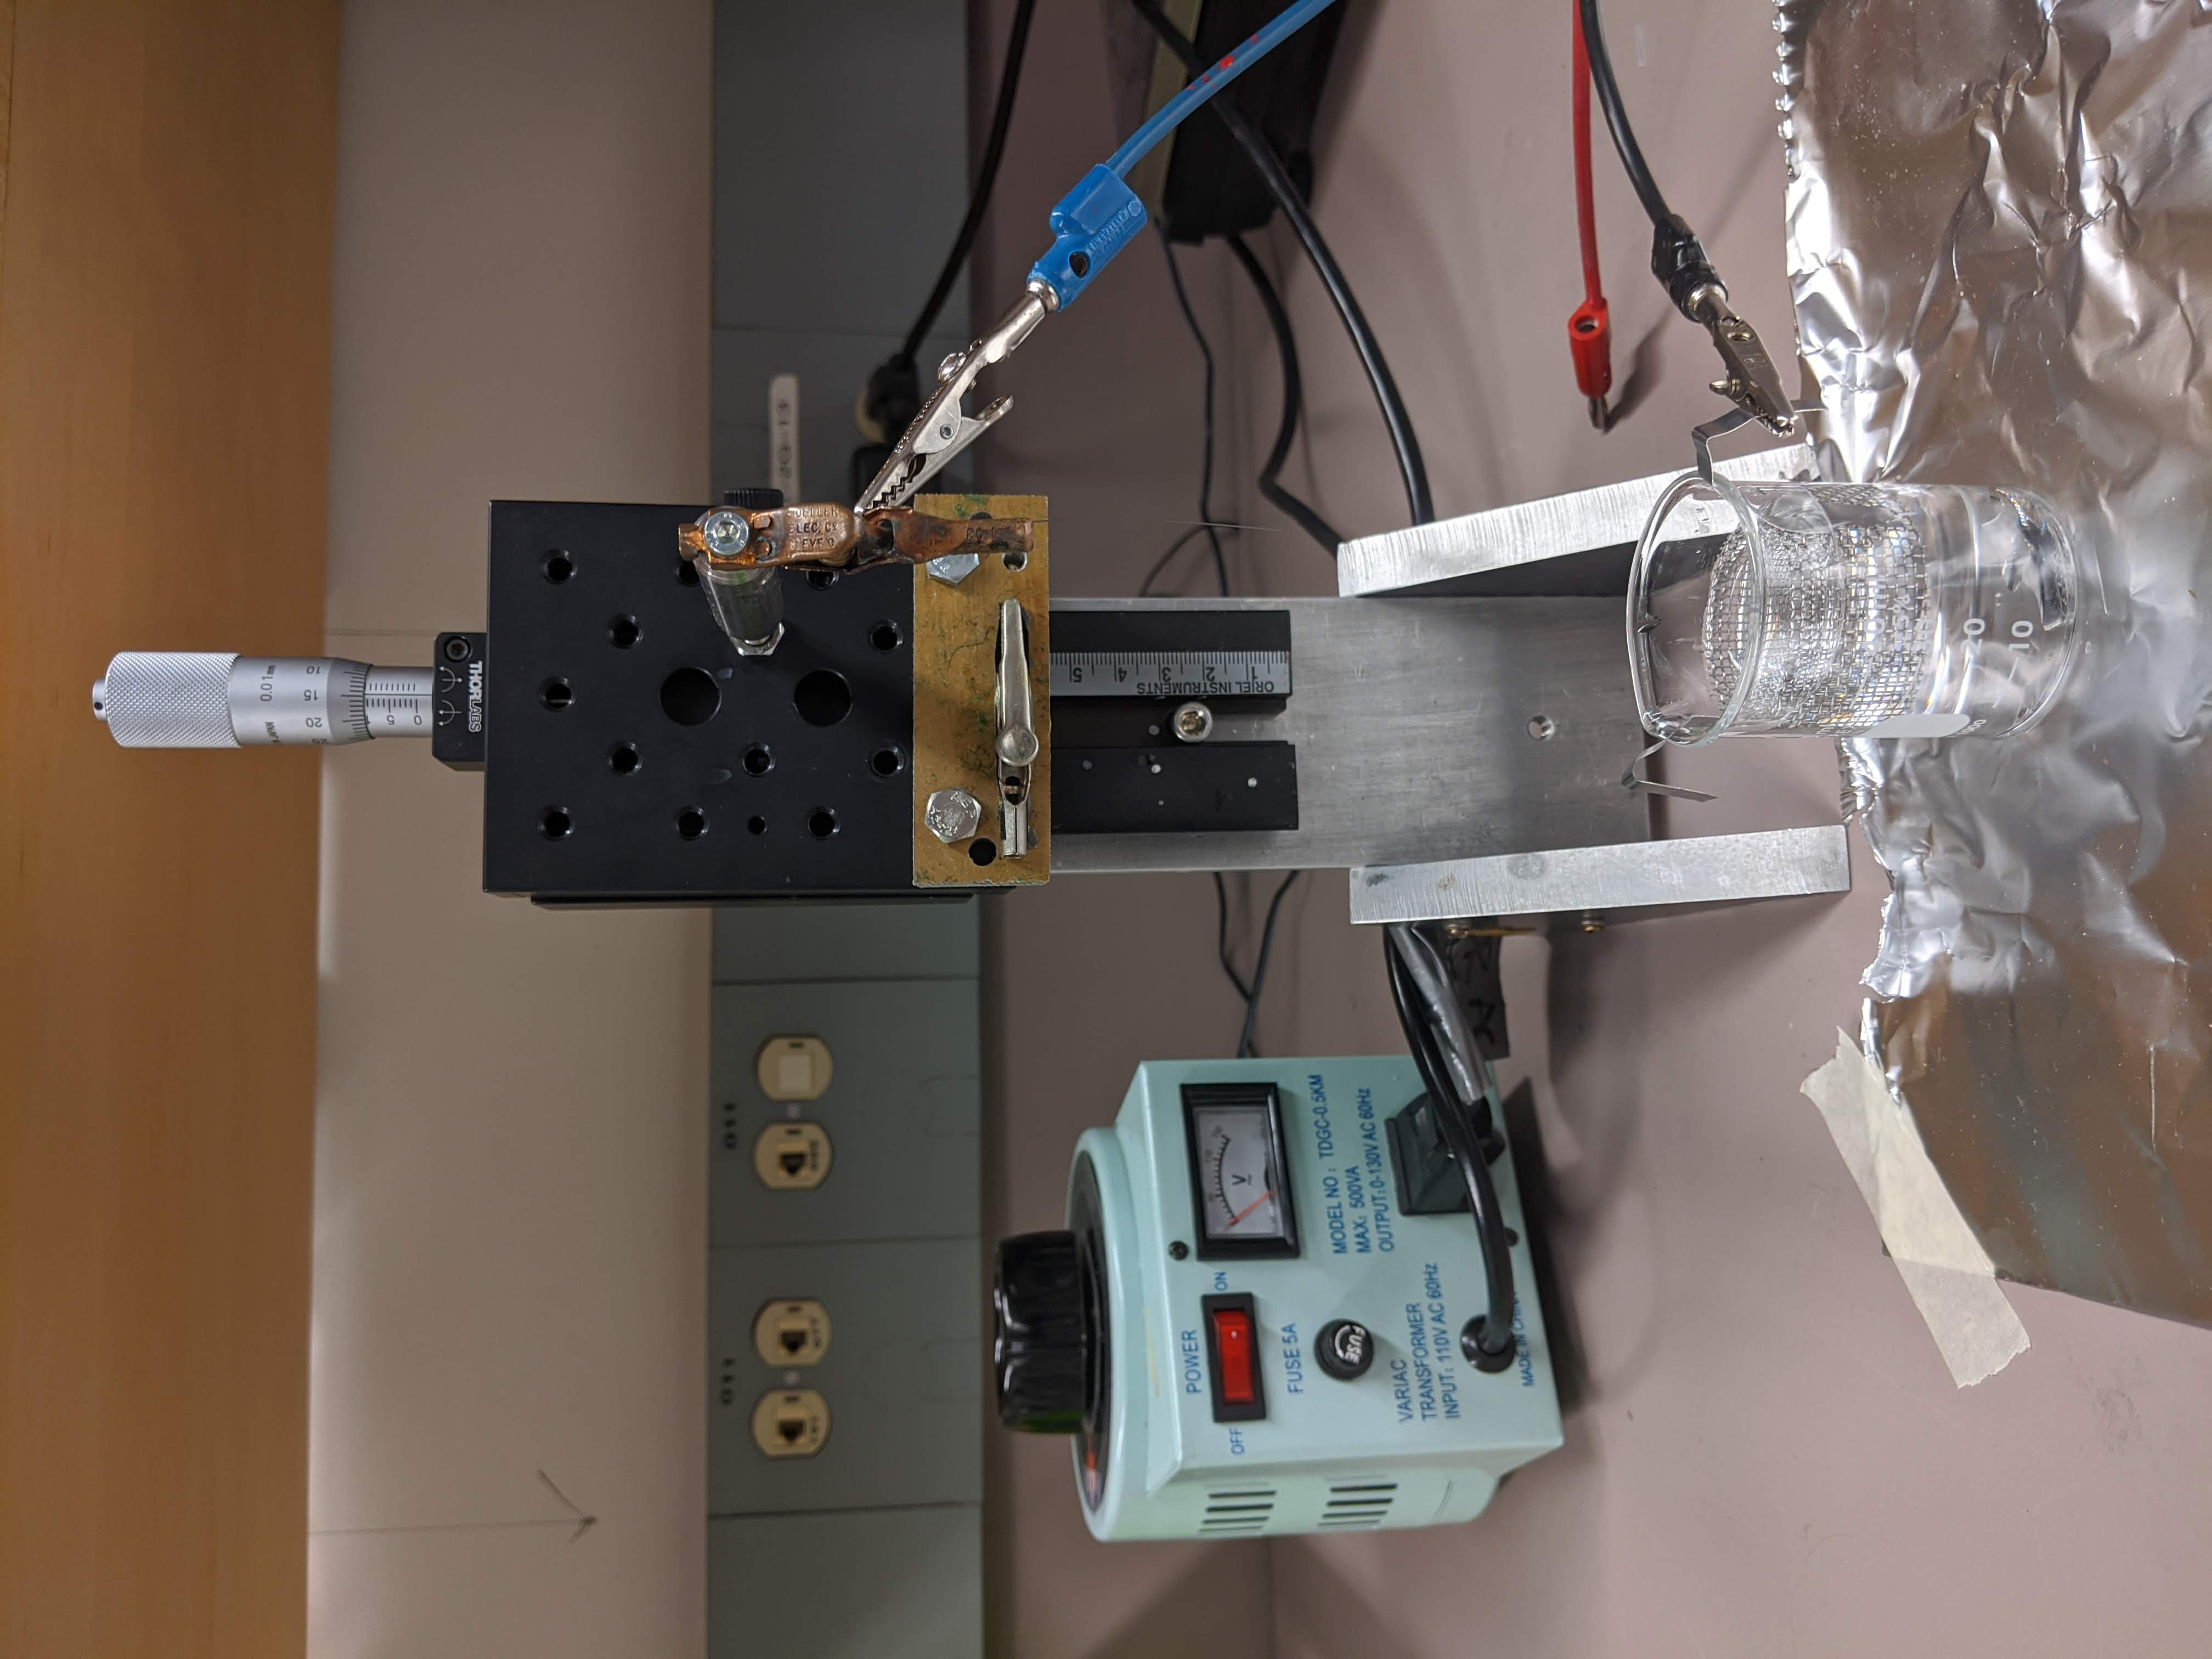
\includegraphics[width=3in,angle=-90]{pictures/etching.jpg}
    \caption{\FIXME{show hmat-tz data}}
    \label{fig:oled:hmat-tz}
\end{figure}

\begin{figure} [h]
    \centering
    %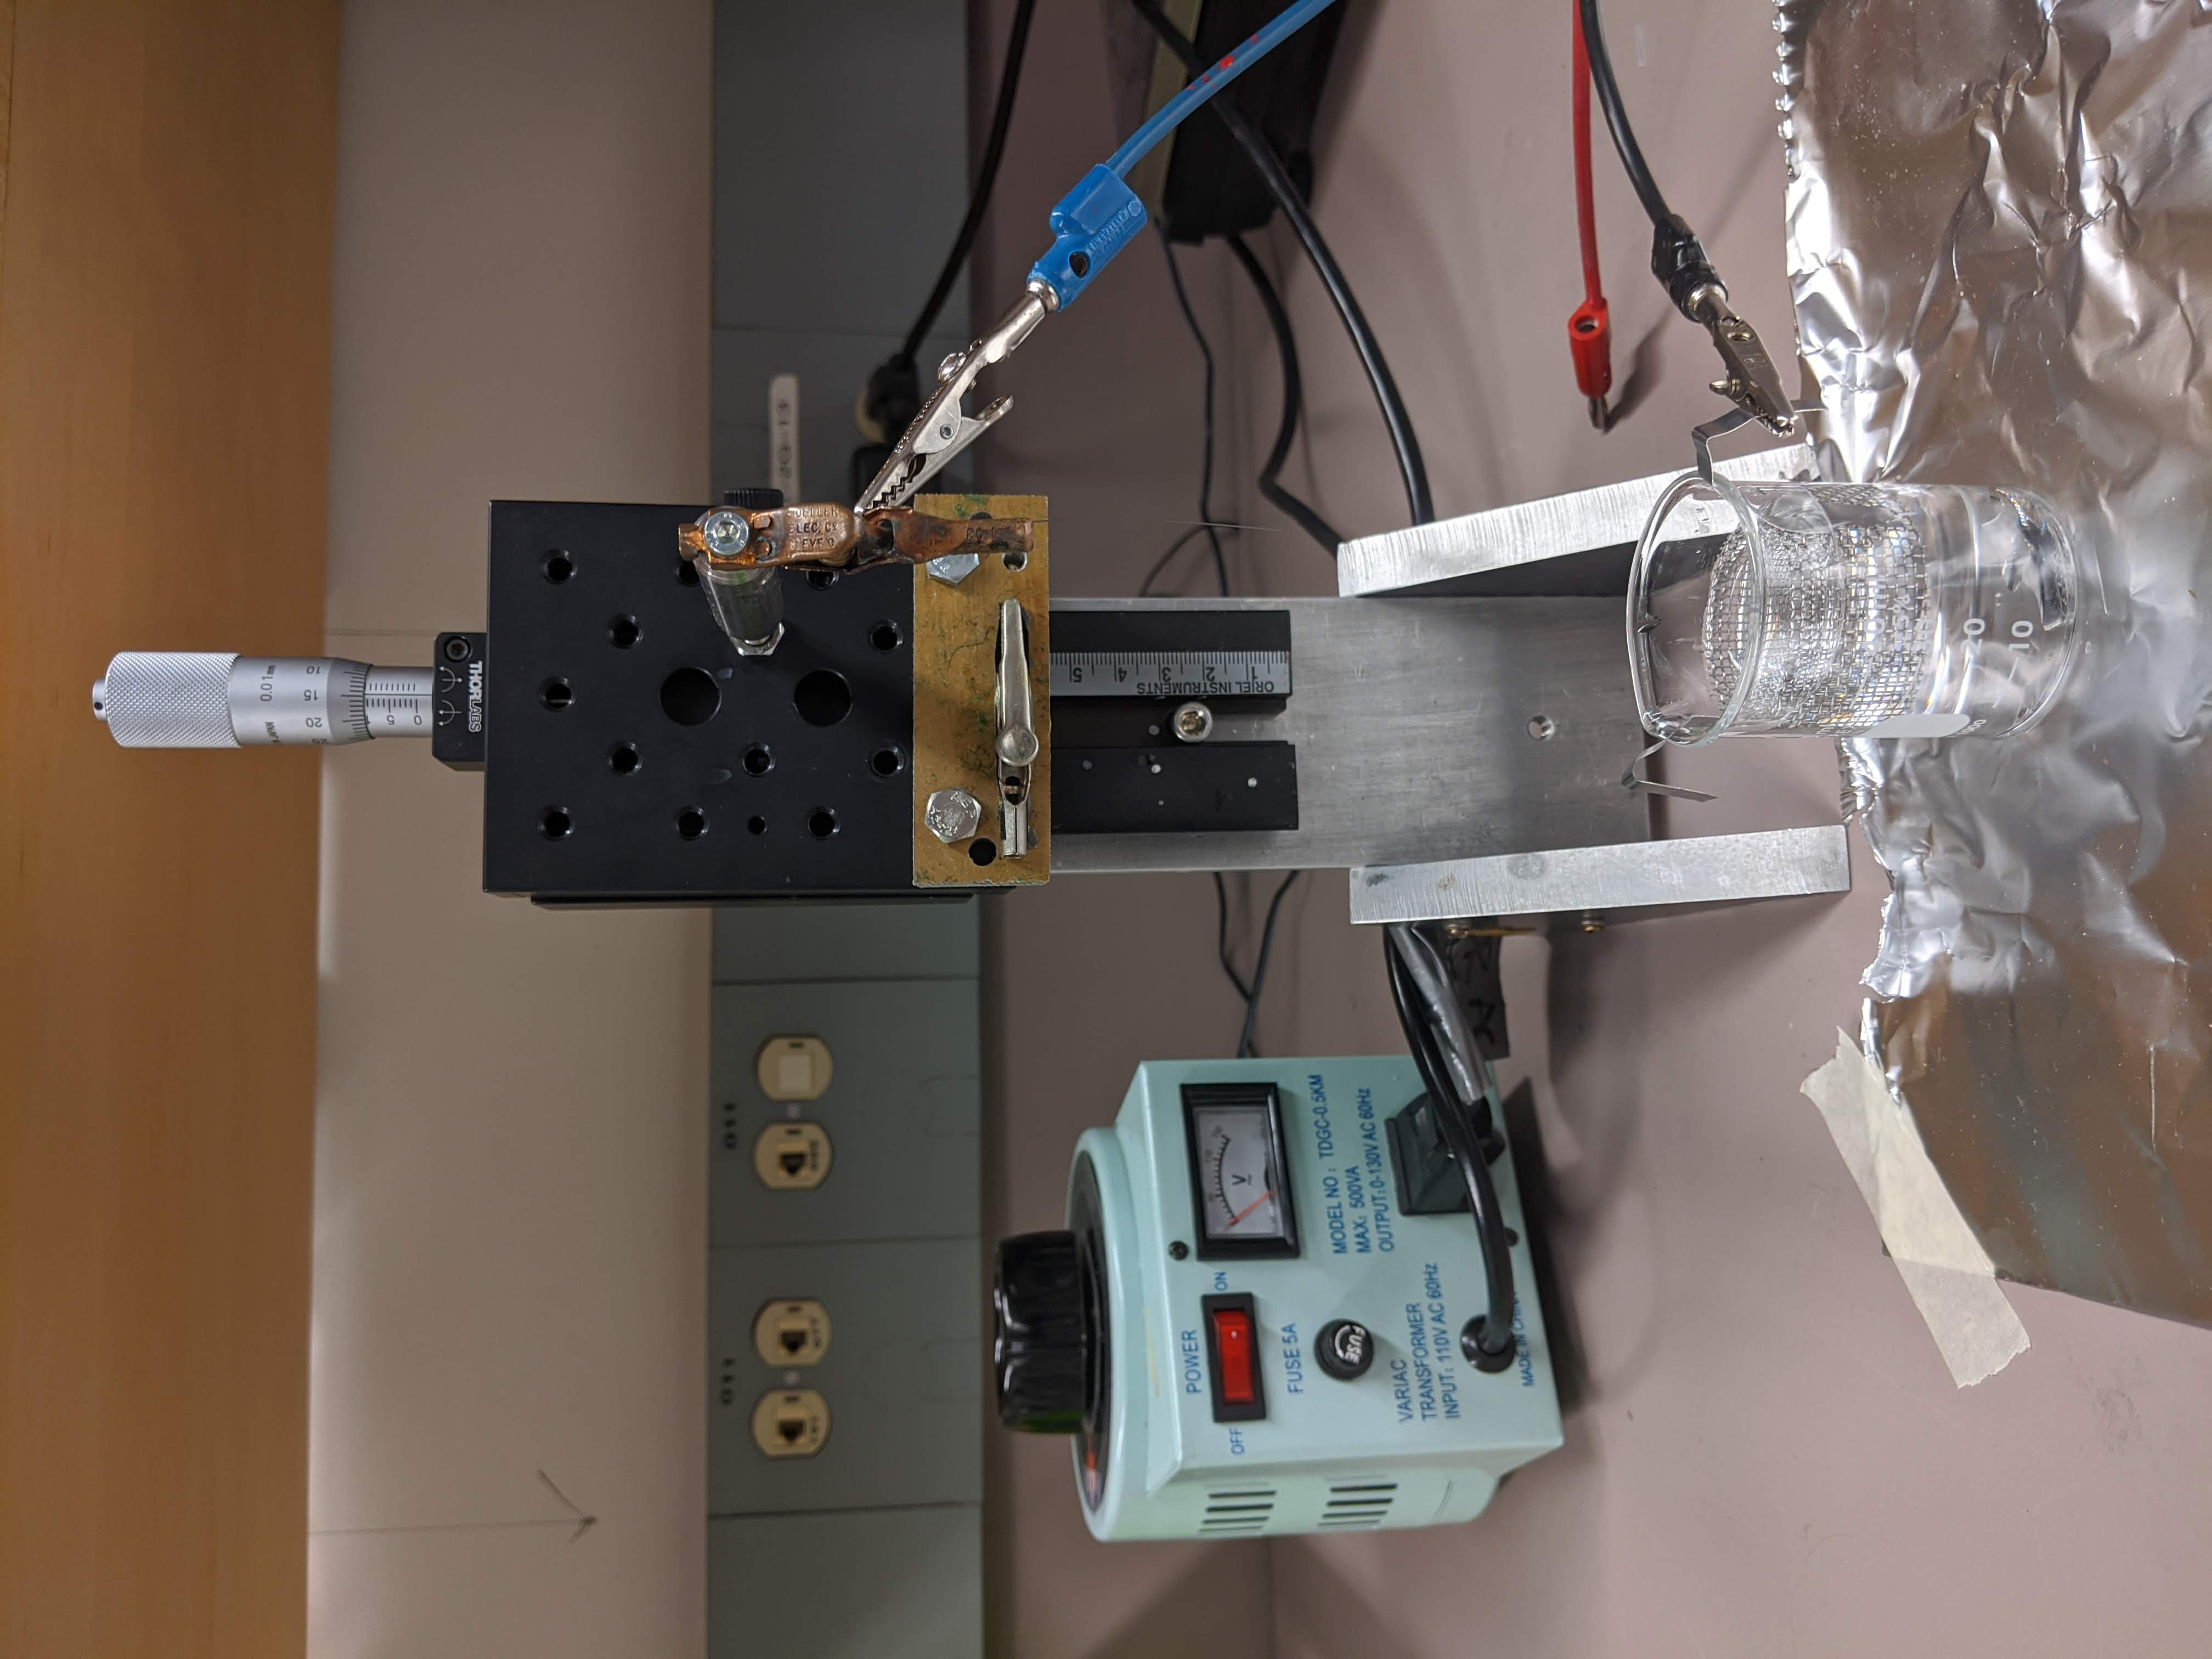
\includegraphics[width=3in,angle=-90]{pictures/etching.jpg}
    \caption{\FIXME{show hmat-hz data}}
    \label{fig:oled:hmat-hz}
\end{figure}

For each of the molecules, there is qualitative agreement in the molecular orbital distribution between the \ac{STS} and the \ac{DFT}---the \ac{HOMO} state is localized on the \ac{HMAT}, while the \ac{LUMO} state is localized on the acceptor group. In the case of \ac{HMAT-HZ}, the LUMO and the LUMO+1 were both imaged in \ac{STS}, and, as seen in the \ac{DFT} result, both were localized primarily on the heptazine.

The experimental and theoretical band gaps for each molecule are summarized in \autoref{tab:oled:bandgaps} and \autoref{fig:oled:bandgap-diagram}. The exact band gap energies do not correspond between \ac{DFT} and \ac{STS}. This is expected, as the \ac{DFT} calculations do not account for the interactions between the molecule and substrate. The \ac{STS} experiments were performed without an insulating NaCl layer, so the molecular orbital energies experience significant shifts.

\begin{table} [h]
\begin{center}
    \begin{tabular}{|c|c|c|} 
    \hline
        Molecule  &  DFT band gap (eV)  &  STS band gap (eV) \\
        \hline
        HMAT     &    4.45   &  --- \\
        HMAT-O   &    3.45   & 3.95 \\
        HMAT-TZ  &    3.28   & 2.60 \\
        HMAT-HZ  &    2.54   & 2.45 \\
        \hline
    \end{tabular}
    \caption{\FIXME{caption this, values may be different with norm didv}}
    \label{tab:oled:bandgaps}
    \end{center}
\end{table}

In both the \ac{DFT} and \ac{STS}, there is a clear trend in the HOMO-LUMO gap of each of the \ac{HMAT} derivatives. With the addition of increasingly electronegative species (with increasing number of \ch{O} and \ch{N} atoms), the electron affinity of the molecule increases, and the \ac{LUMO} is lowered in energy (\autoref{fig:oled:bandgap-diagram}). The \ac{HOMO} experiences no shift in energy relative to the Fermi level.

\begin{figure} [h]
    \centering
    %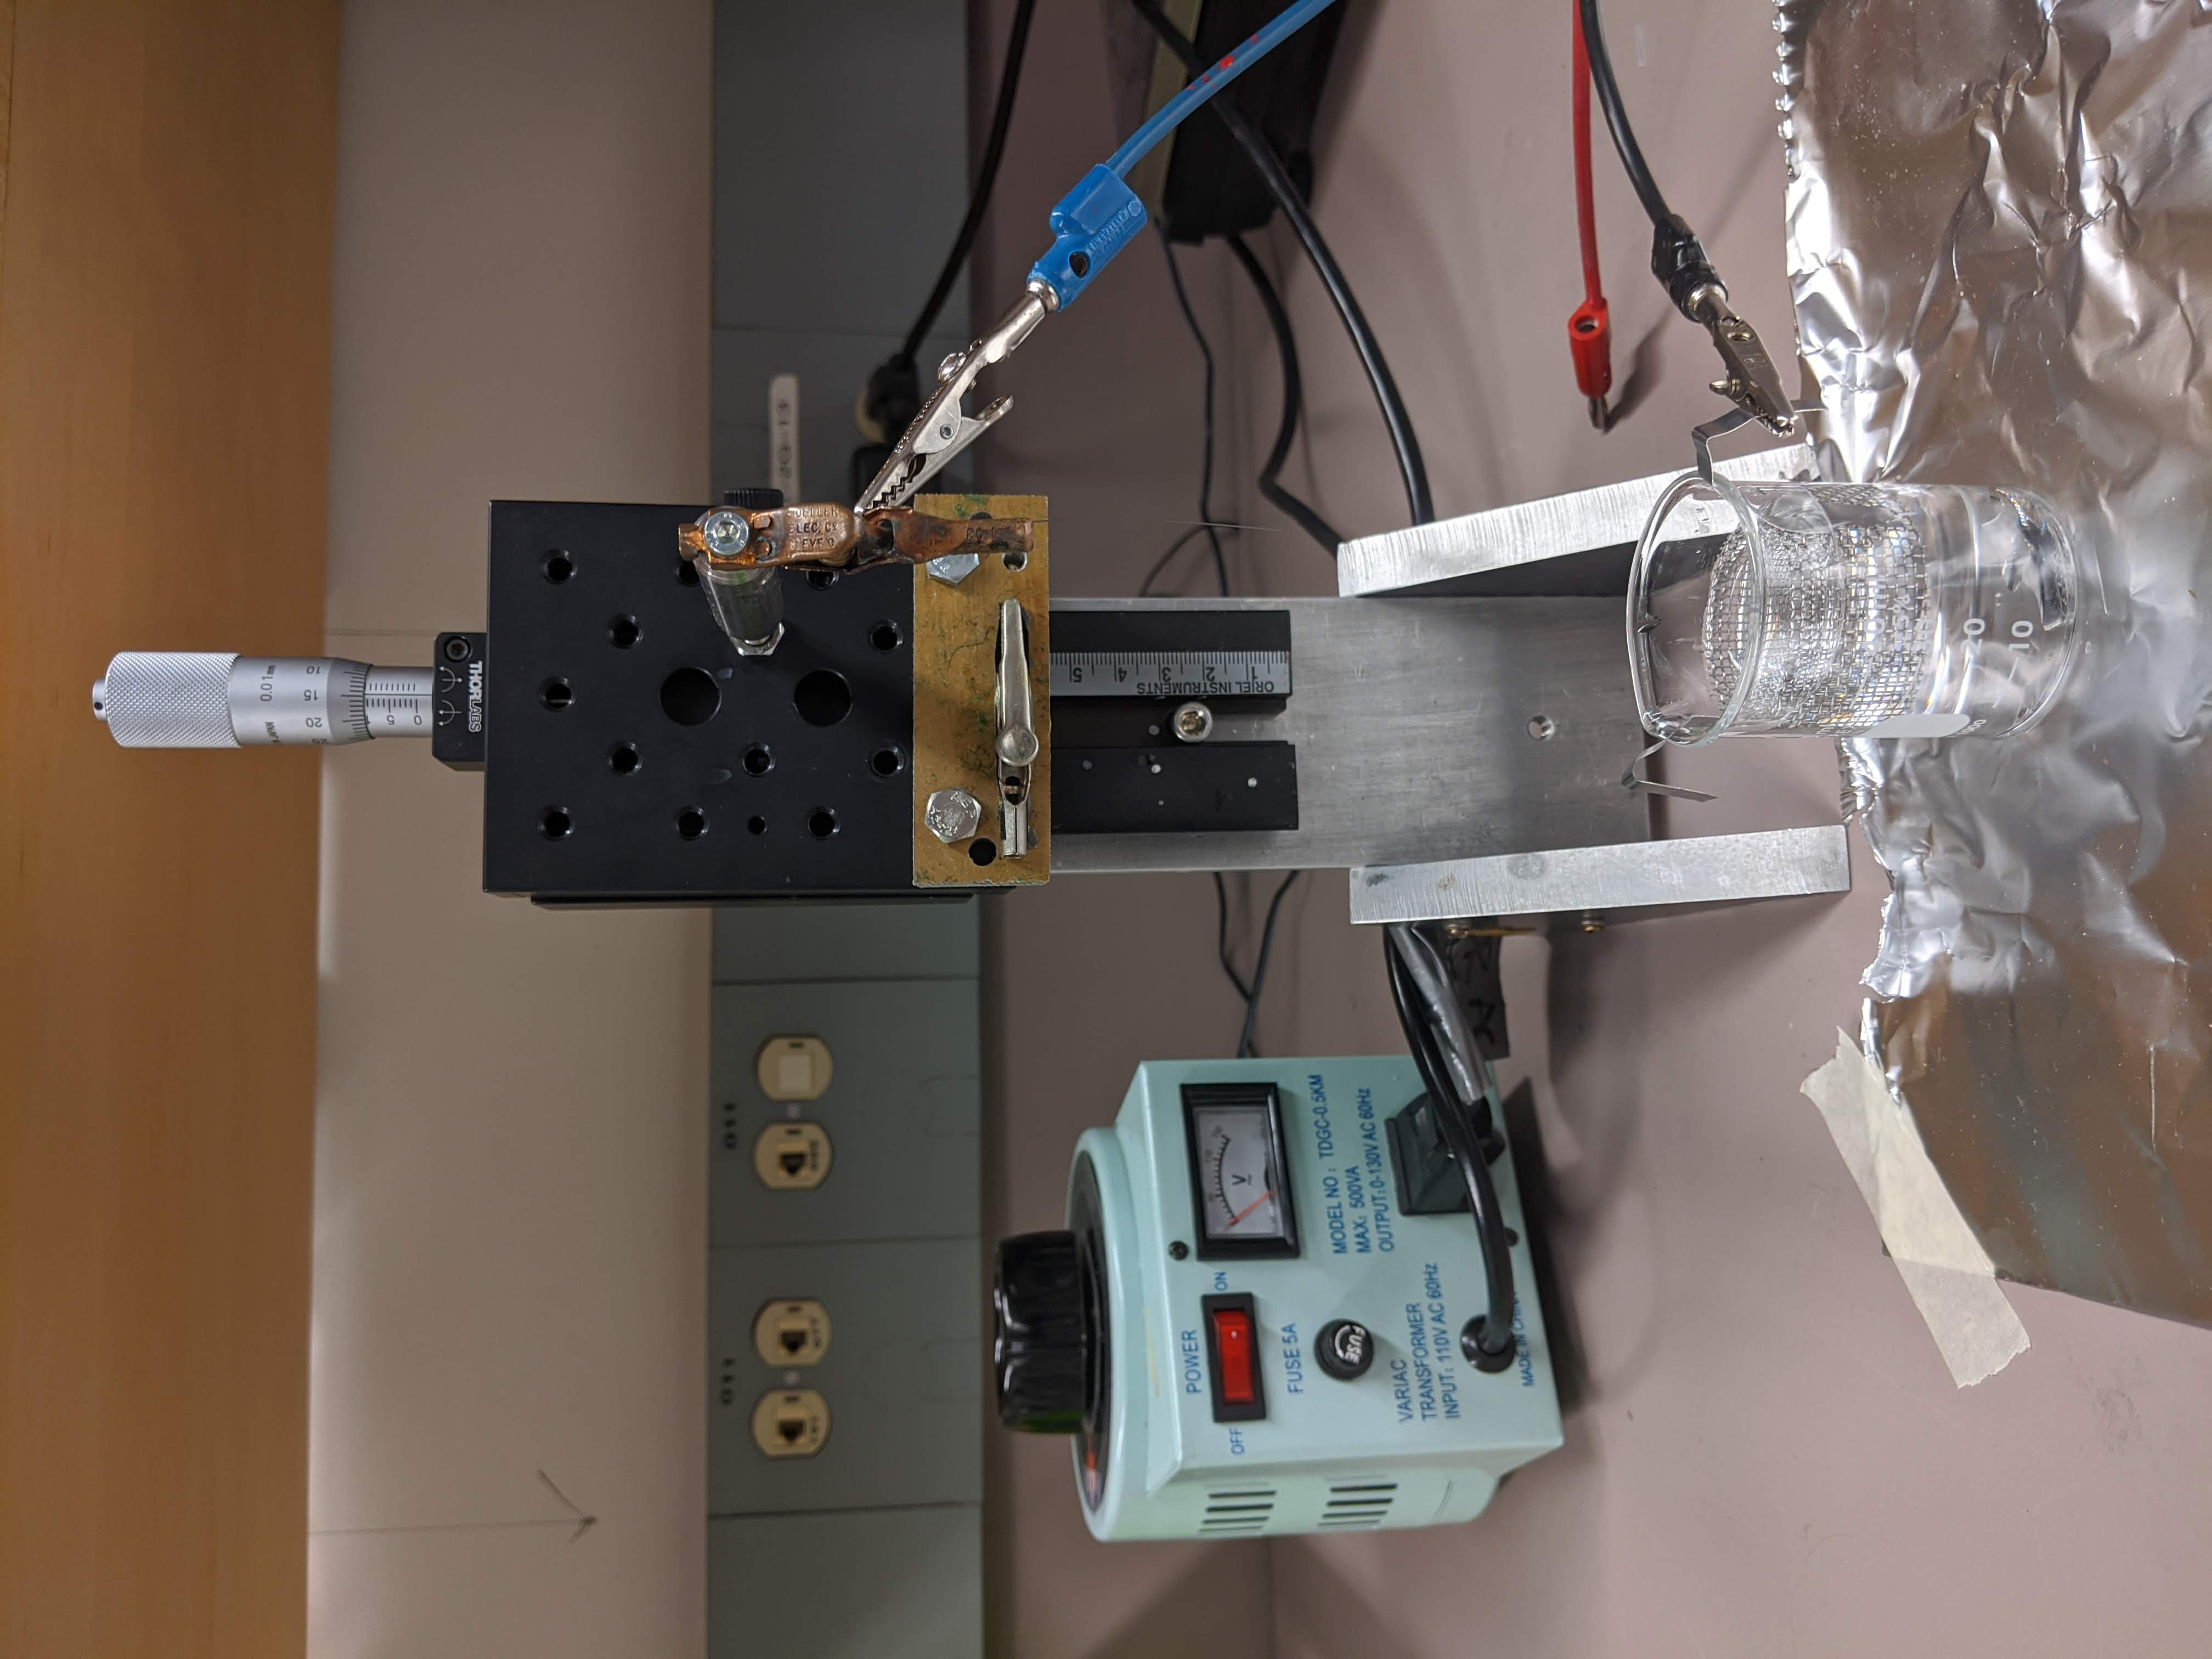
\includegraphics[width=3in,angle=-90]{pictures/etching.jpg}
    \caption{\FIXME{band gap shrinking diagram}}
    \label{fig:oled:bandgap-diagram}
\end{figure}

No attempts were made to perform \ac{SPM} on these molecules on an insulating NaCl layer due to the fragility and instability of the molecules at higher biases. At tip-sample biases $|V_b| > \SI{2.5}{V}$, the molecules would shift on the surface, and the bonds between the \ac{HMAT} and the functional groups occasionally dissociated. The decoupling of the molecules from the substrate would have resulted in larger band gaps, meaning the molecular orbitals would likely not have been accessible by \ac{SPM}.



\section{{STML} study of HMAT derivatives}

While the molecules were not dissociated from the substrate by a bilayer of NaCl, \ac{STML} was attempted for \ac{HMAT-O} and \ac{HMAT-HZ}. With successfully resolved molecular states in the \ac{STS}, we hypothesized that the bulky methyl groups (six on each \ac{HMAT}) may have sterically disscoiates the molecule from the underlying Ag(111).

However, with the Ag tip parked on the molecule at parameters up to \SI{3}{V}/\SI{200}{pA}/\SI{360}{s}, no molecular luminescence was detected, only the plasmonic emission. We also attempted to obtain an absorption spectra by exciting plasmonic photons near the molecule, a technique demonstrated in the past on ZnPc \cite{zhang2017sub}, but again, only the plasmonic emission was seen. The same experiments were repeated on Au(111), in an attempt to red-shift the plasmon emission so as to observe the two-photon absorption of the molecules. In all our experiments, no observable \ac{STML} molecular signatures were found from the HMAT-O or HMAT-HZ directly adsorbed on either Ag(111) or Au(111). 

These failed attempts illustrate the importance of dissociation of the molecule from the substrate in \ac{STML}. Metal-molecule coupling results in additional energy pathways that rapidly quench excited states, and any emission signal from the molecule. Additionally, the instability and large band gaps of \ac{HMAT} derivatives make it difficult to inject charges into the electronic orbitals, or to generate high energy plasmonic emissions to form excitons in the material, without the molecules breaking or moving. 




%%%%%
